\frame{
  \frametitle{Representing Collision Sequences}

  \begin{itemize}
    \item Tile the table in the plane for a more powerful representation of the problem
    \item Tiling will reflect the table about each side
    \item After tiling, we only need to deal with straight line trajectories in a tiled plane
  \end{itemize}
}

\frame{
  \frametitle{Tiling Tables}
  \begin{figure}
    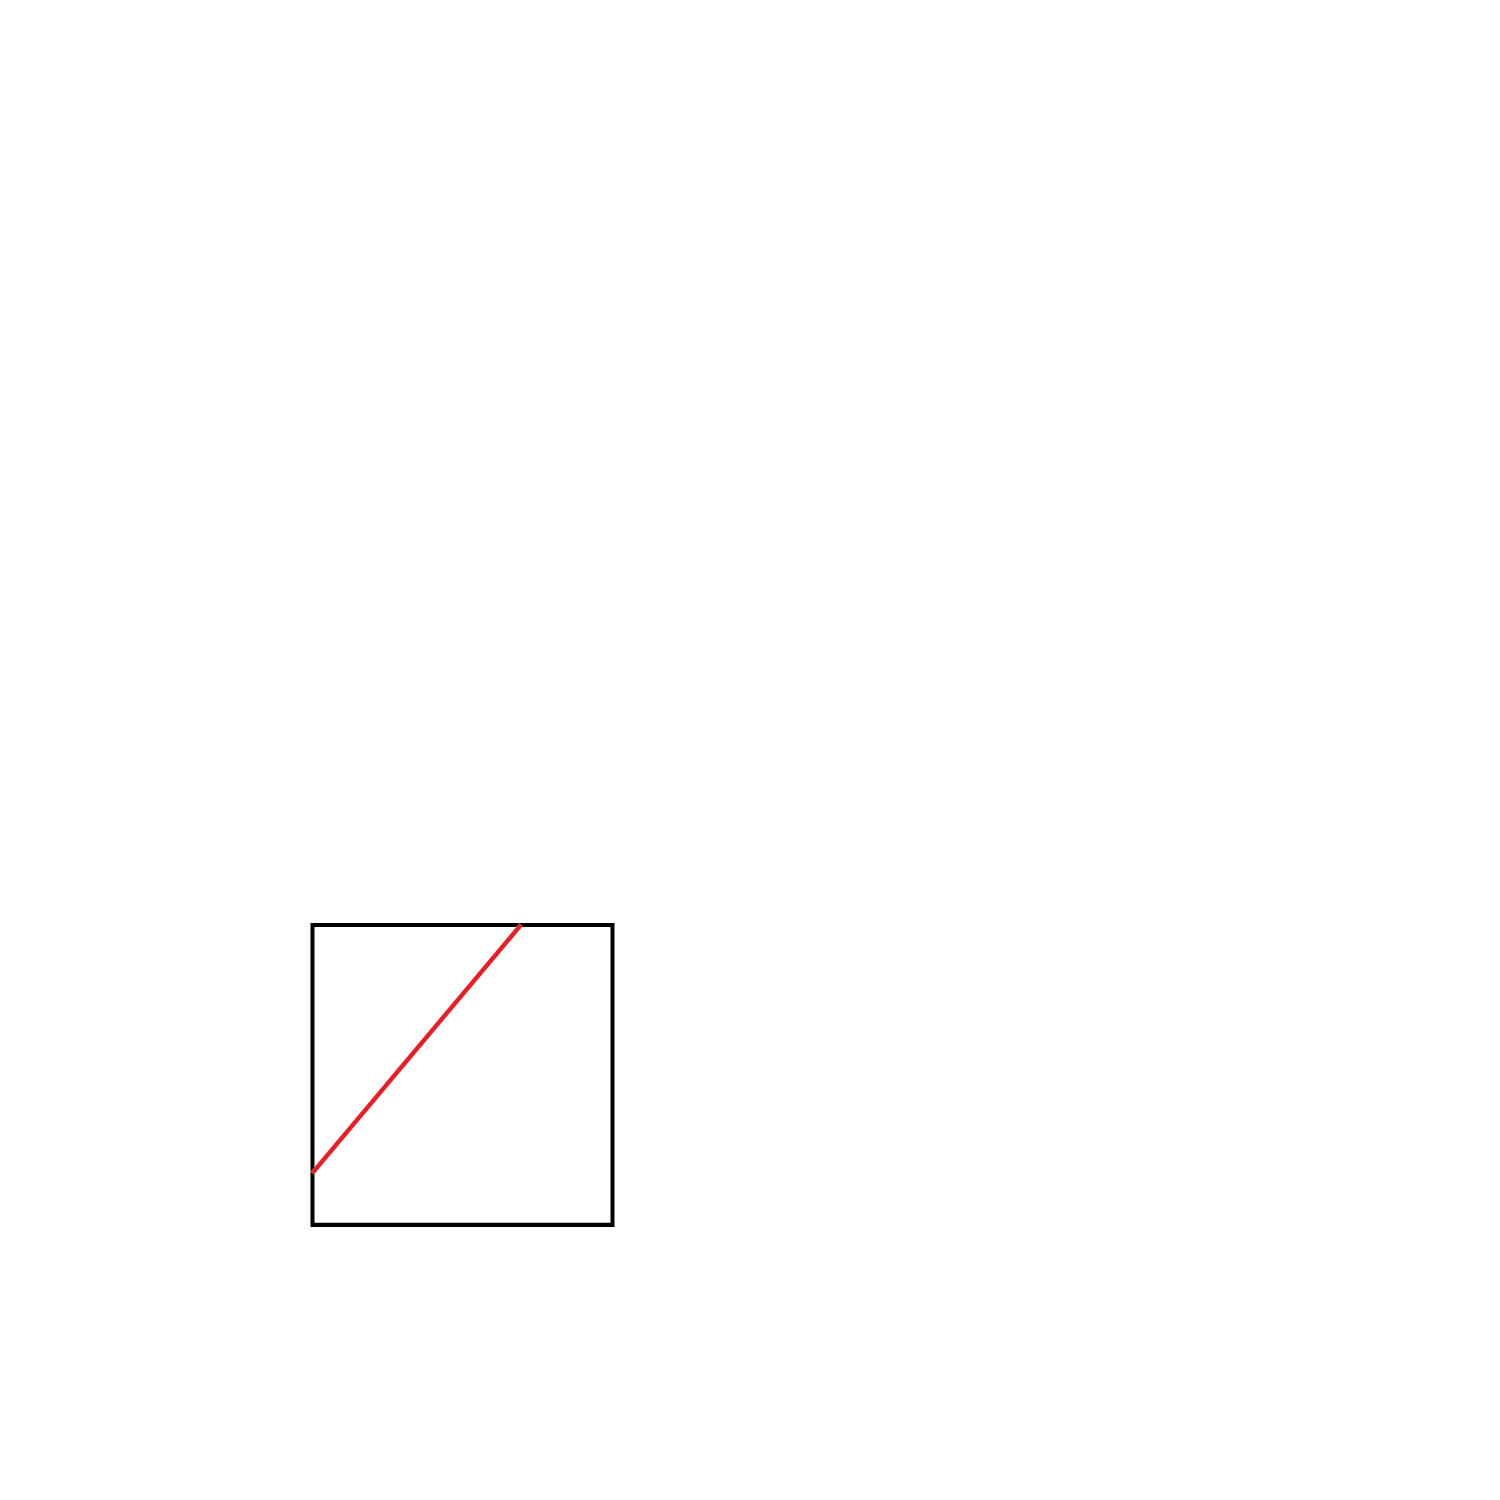
\includegraphics[width=3in]{tiling_(1)-01.png}
  \end{figure}
}
\frame{
  \frametitle{Tiling Tables}
  \begin{figure}
    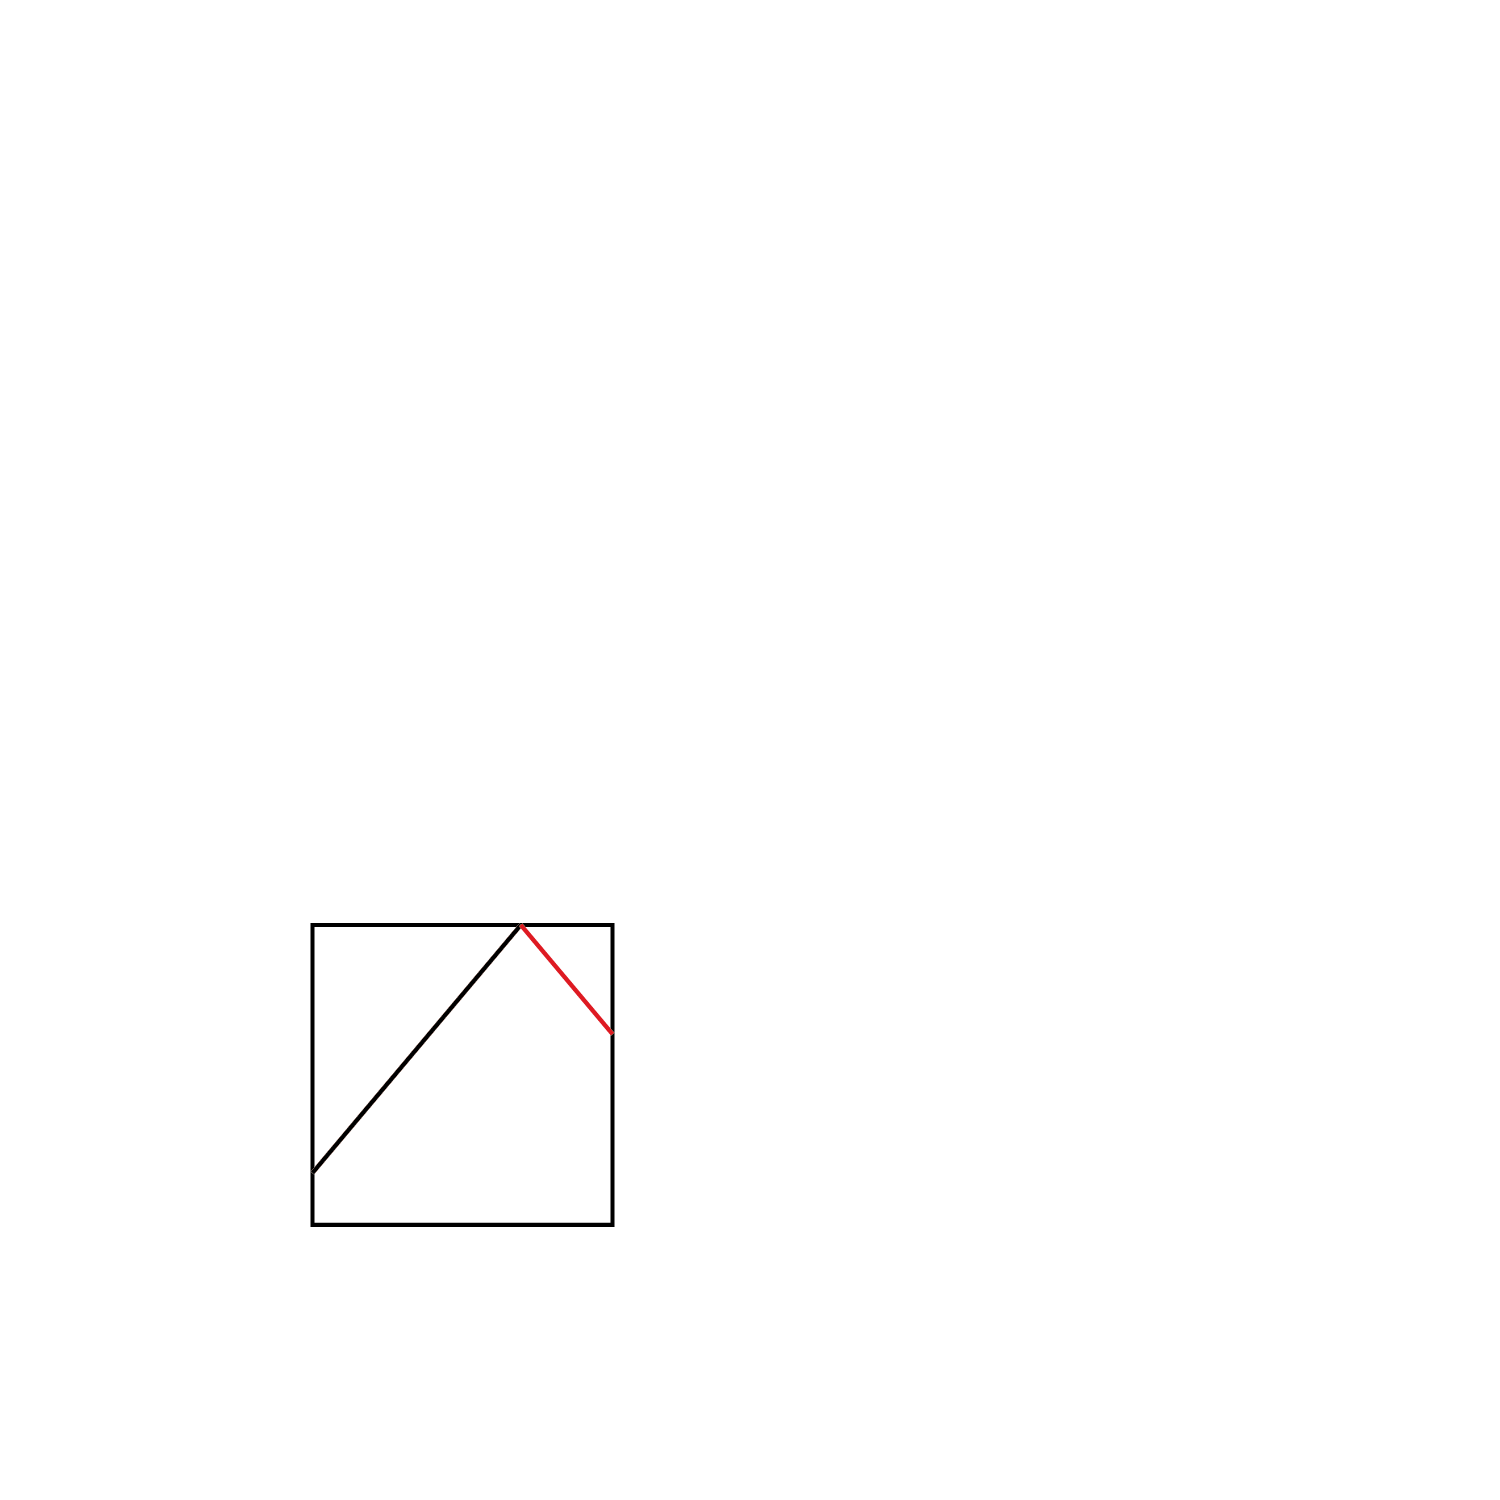
\includegraphics[width=3in]{tiling_(2)-01.png}
  \end{figure}
}
\frame{
  \frametitle{Tiling Tables}
  \begin{figure}
    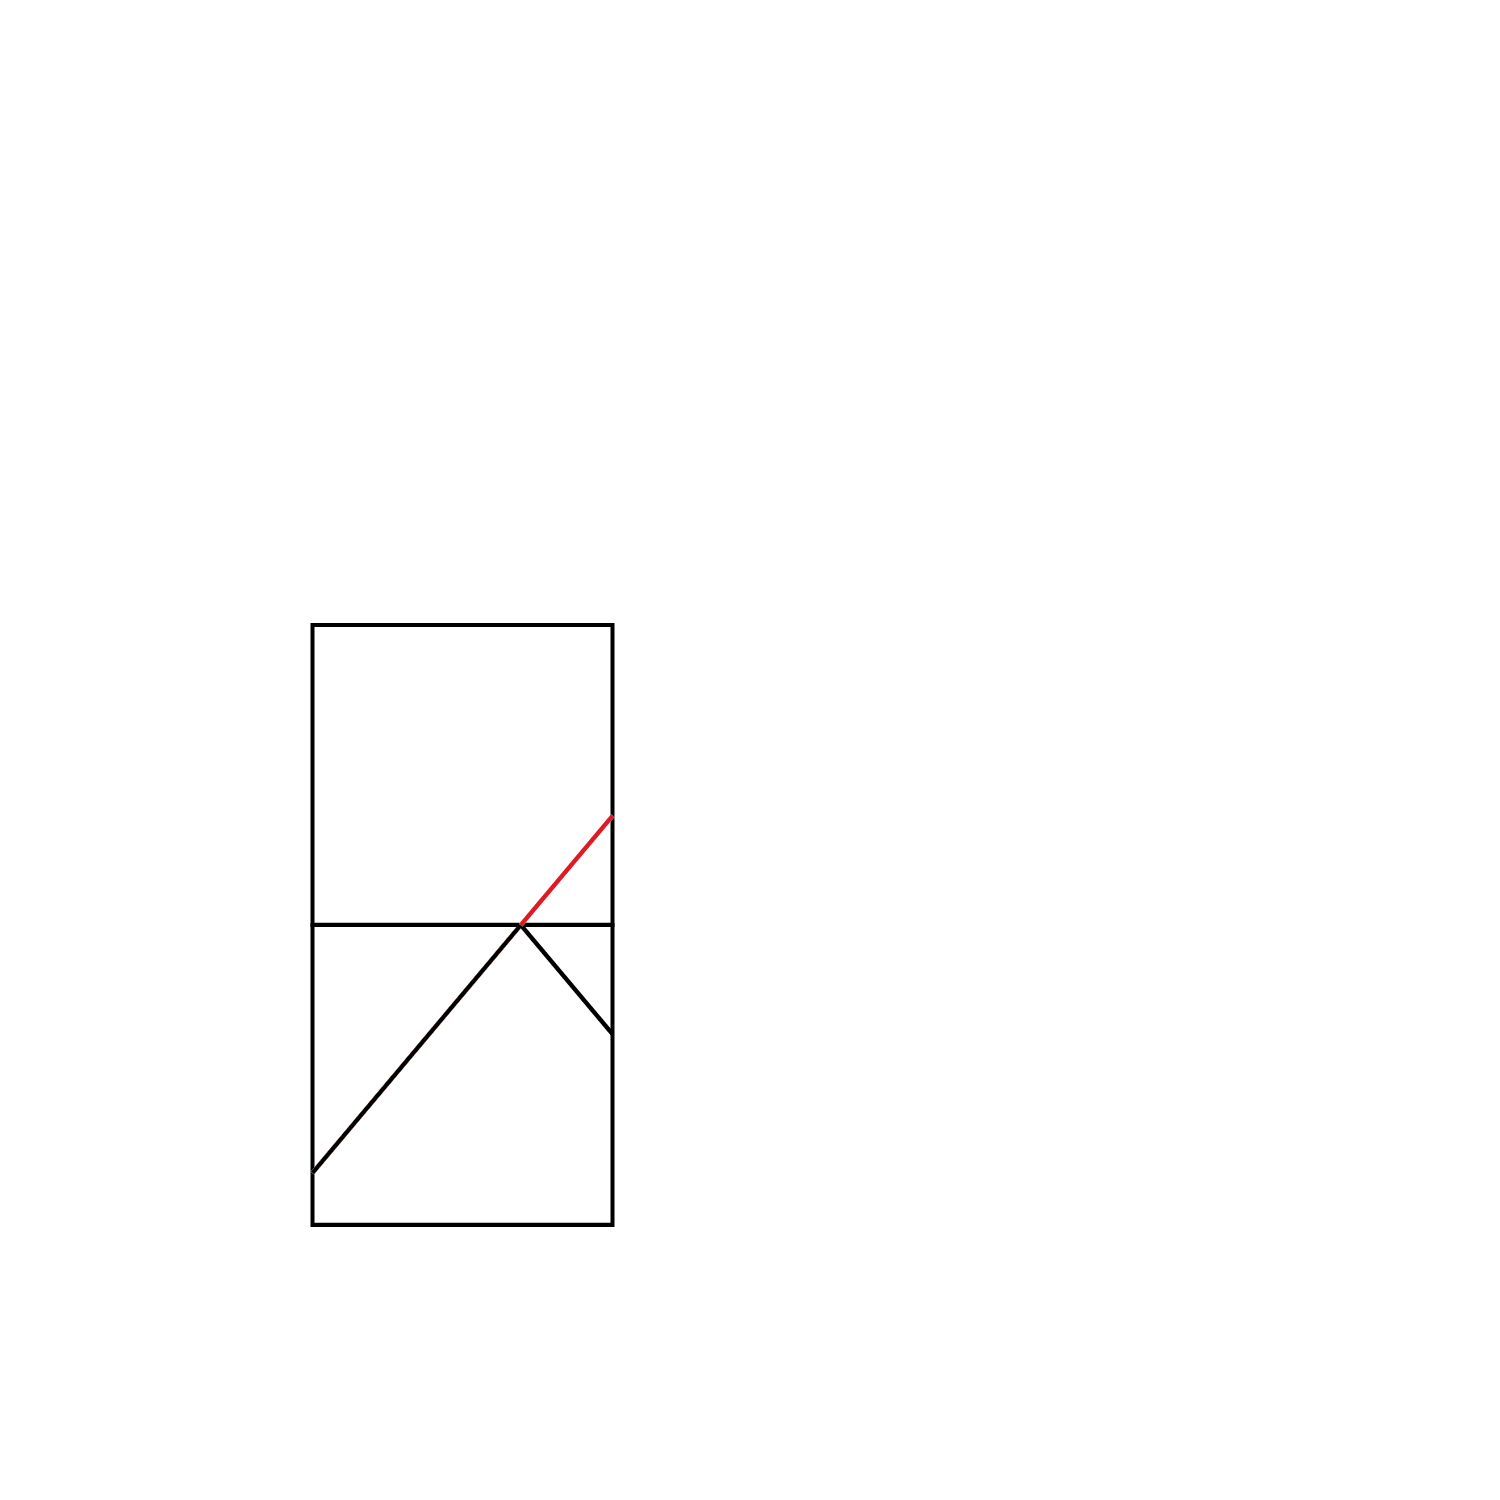
\includegraphics[width=3in]{tiling_(3)-01.png}
  \end{figure}
}
\frame{
  \frametitle{Tiling Tables}
  \begin{figure}
    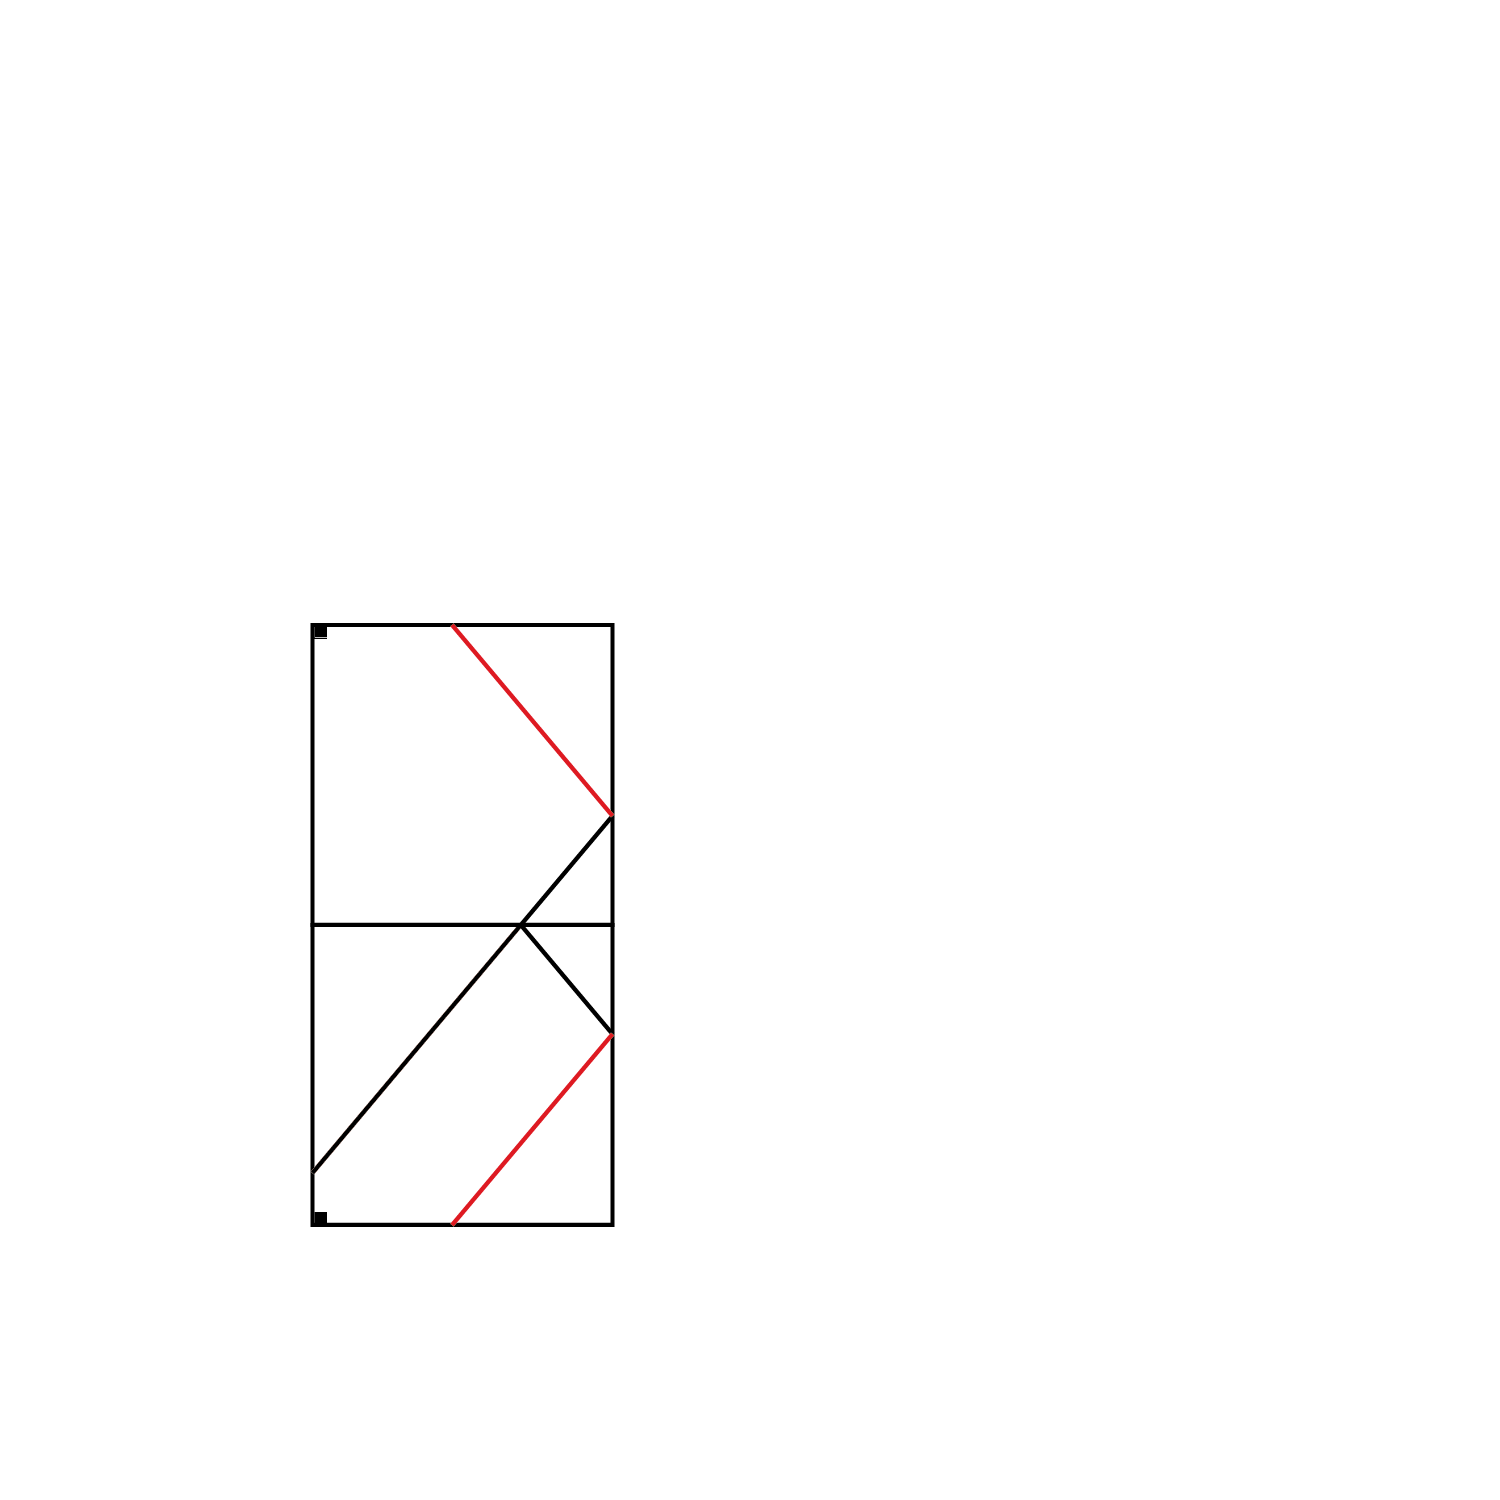
\includegraphics[width=3in]{tiling_(4)-01.png}
  \end{figure}
}
\frame{
  \frametitle{Tiling Tables}
  \begin{figure}
    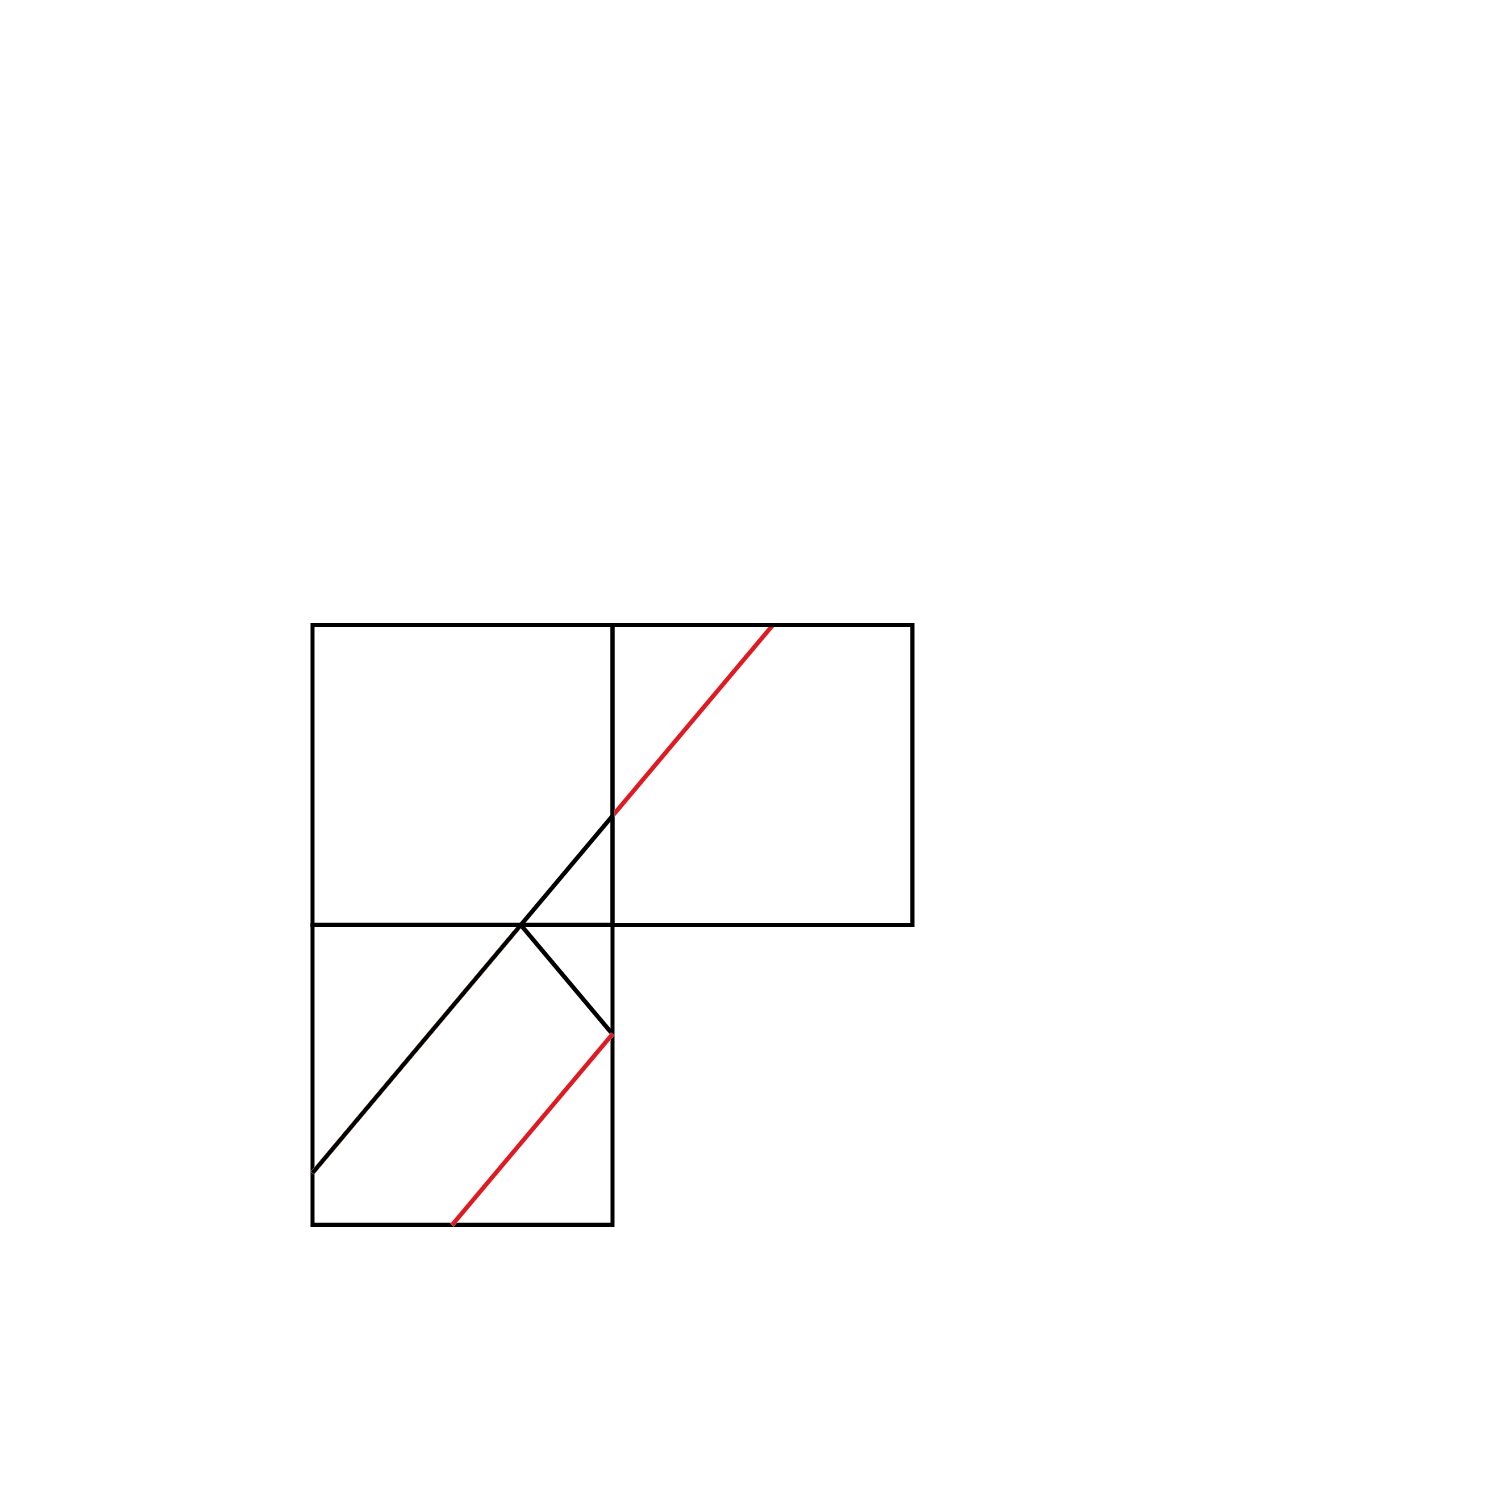
\includegraphics[width=3in]{tiling_(5)-01.png}
  \end{figure}
}
\frame{
  \frametitle{Tiling Tables}
  \begin{figure}
    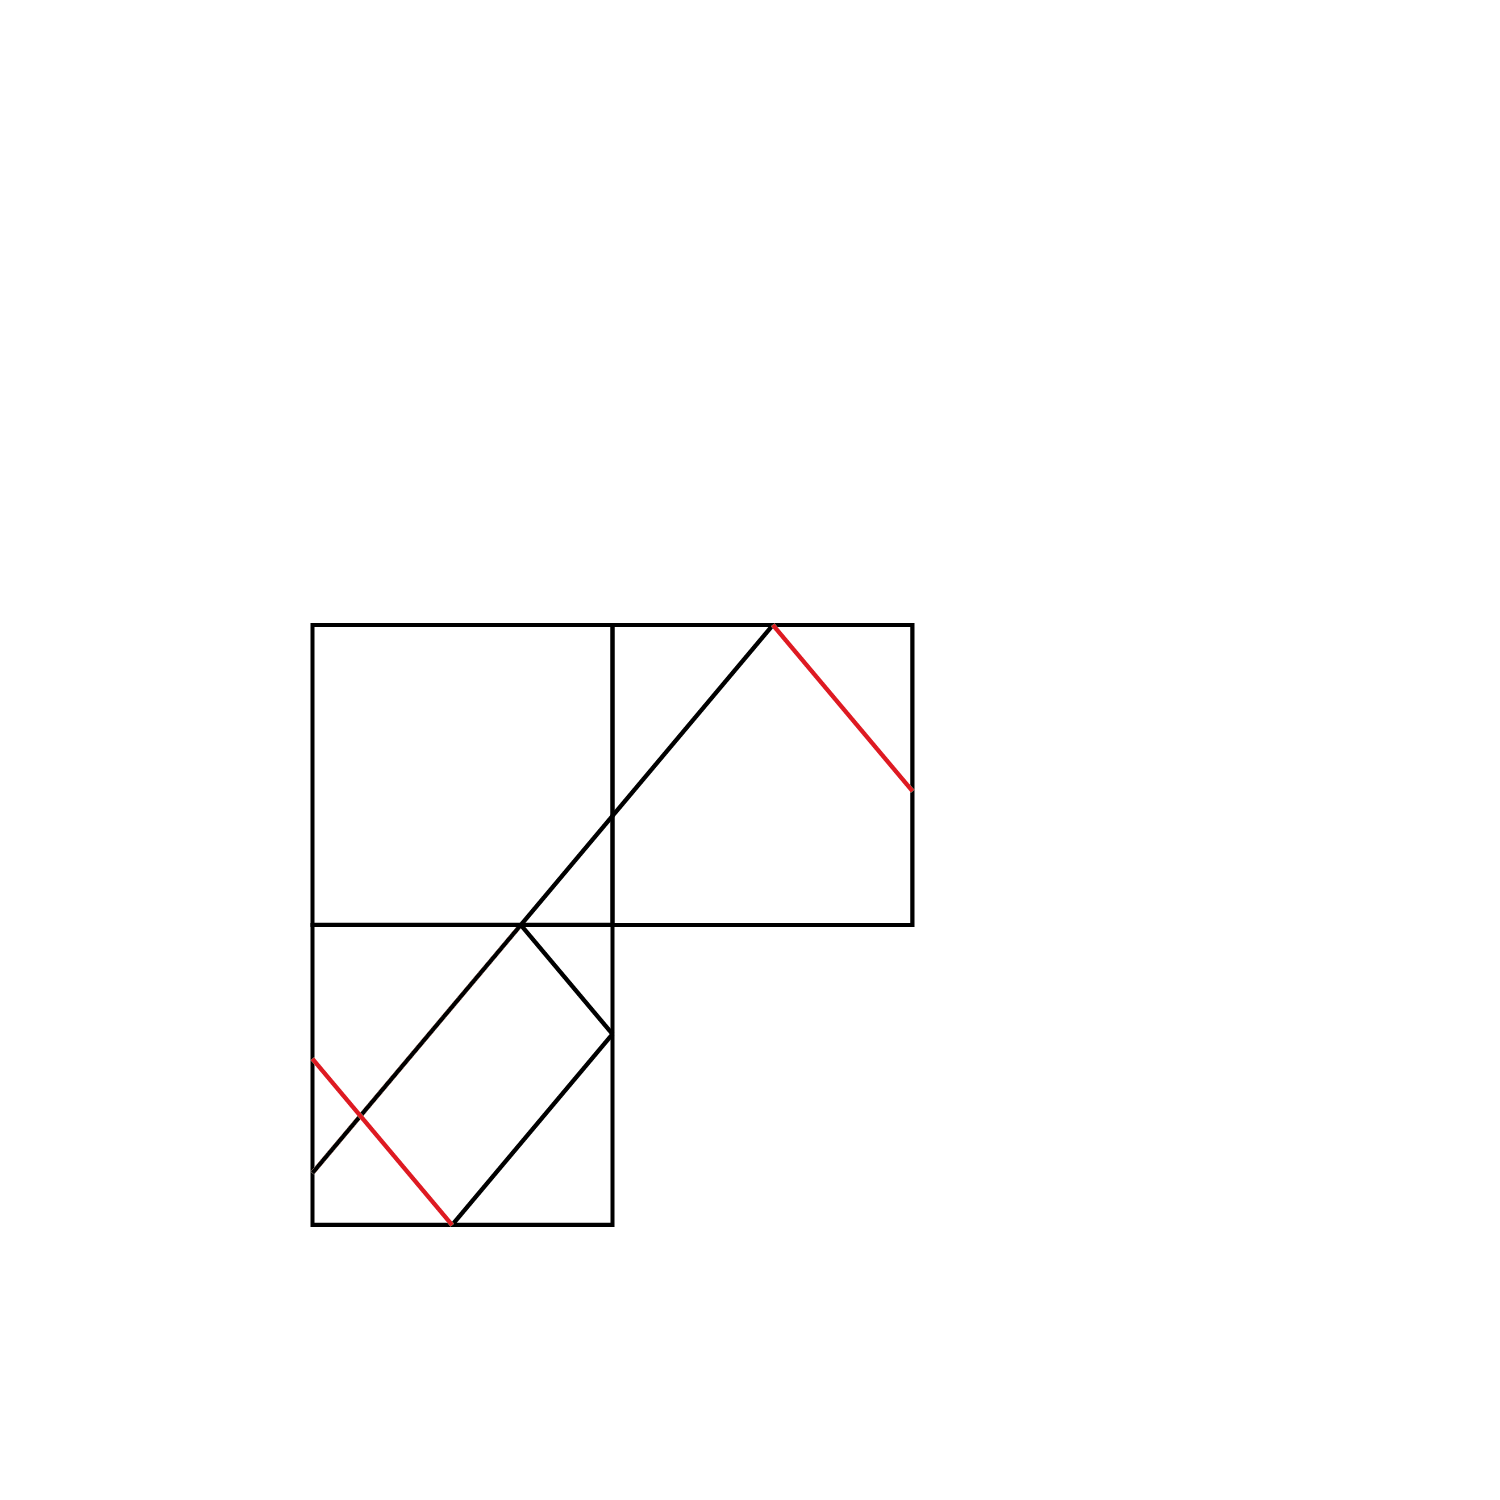
\includegraphics[width=3in]{tiling_(6)-01.png}
  \end{figure}
}
\frame{
  \frametitle{Tiling Tables}
  \begin{figure}
    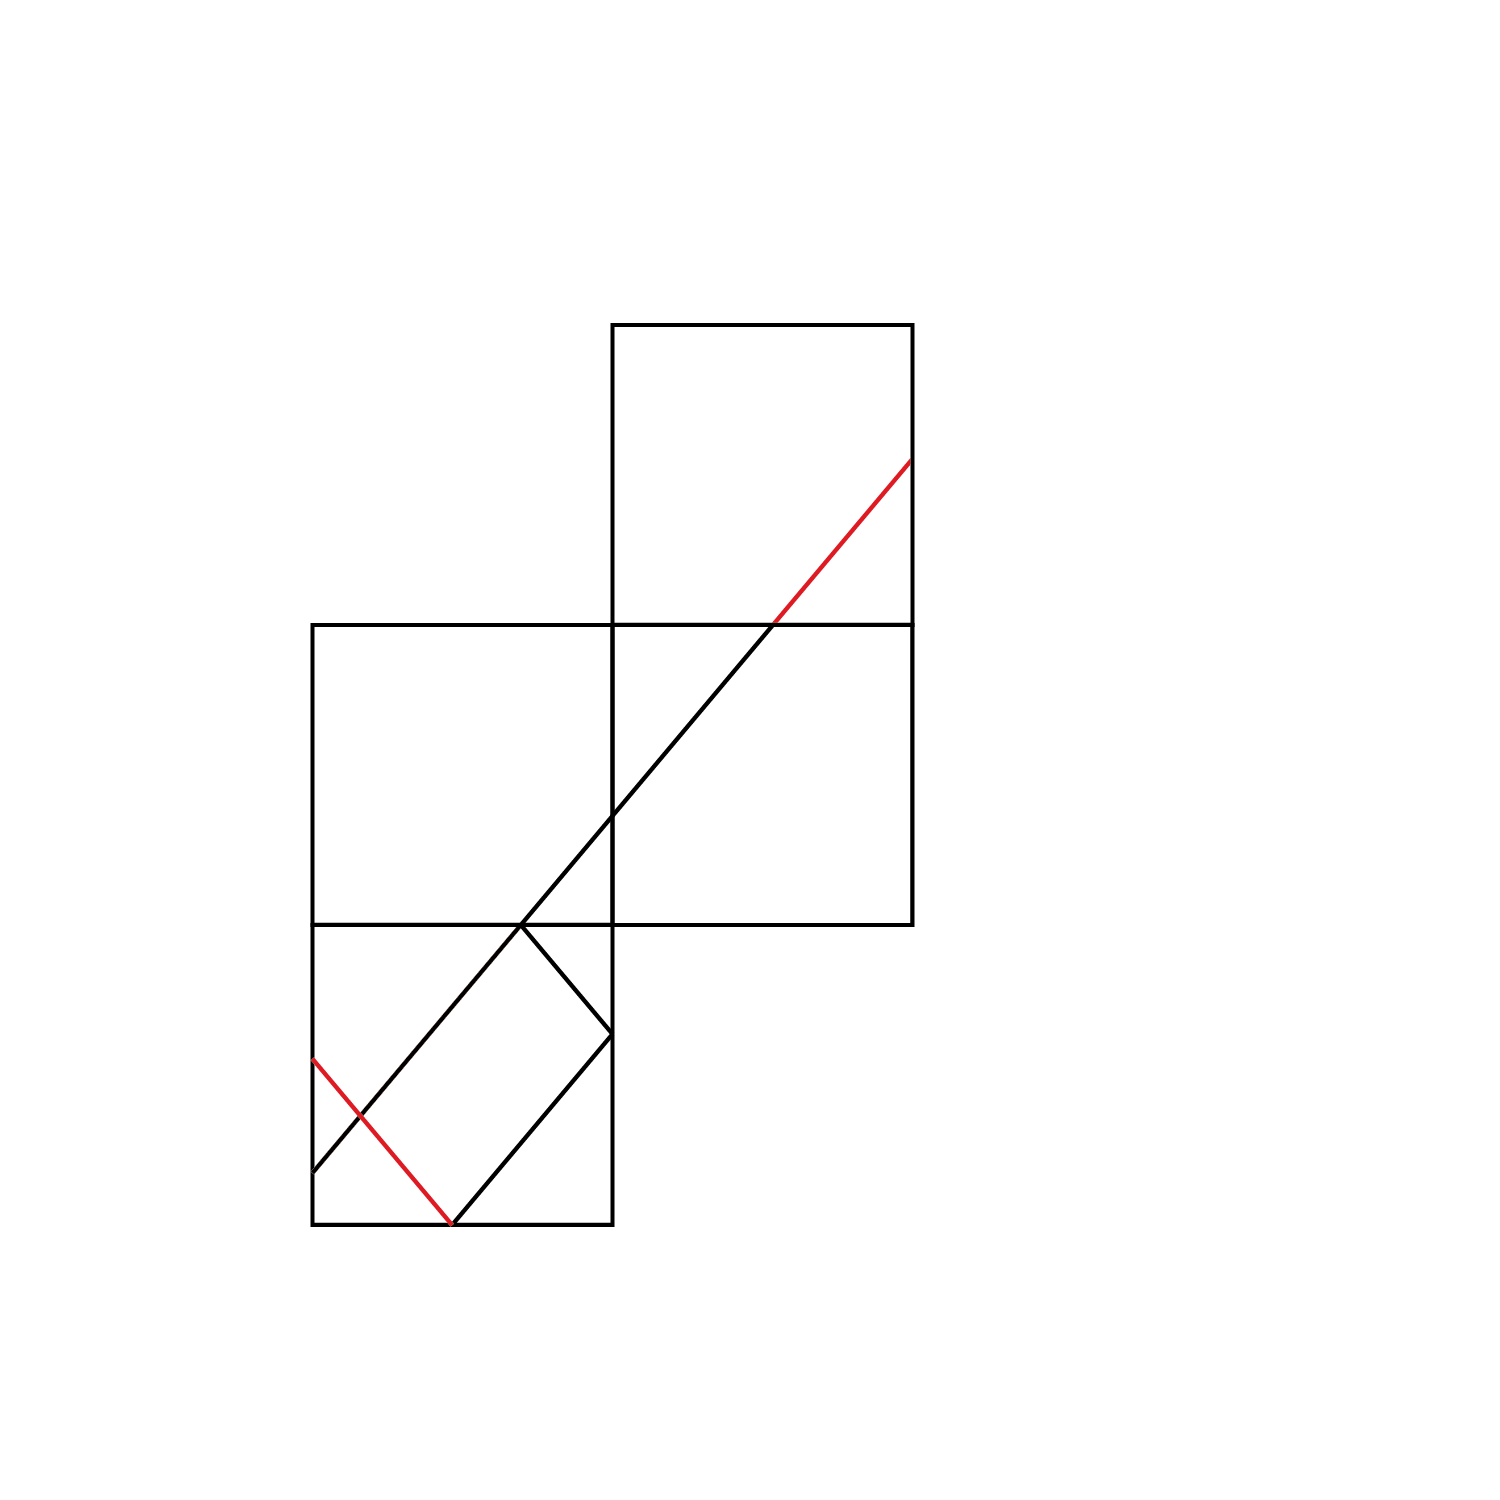
\includegraphics[width=3in]{tiling_(7)-01.png}
  \end{figure}
}
\frame{
  \frametitle{Tiling Tables}
  \begin{figure}
    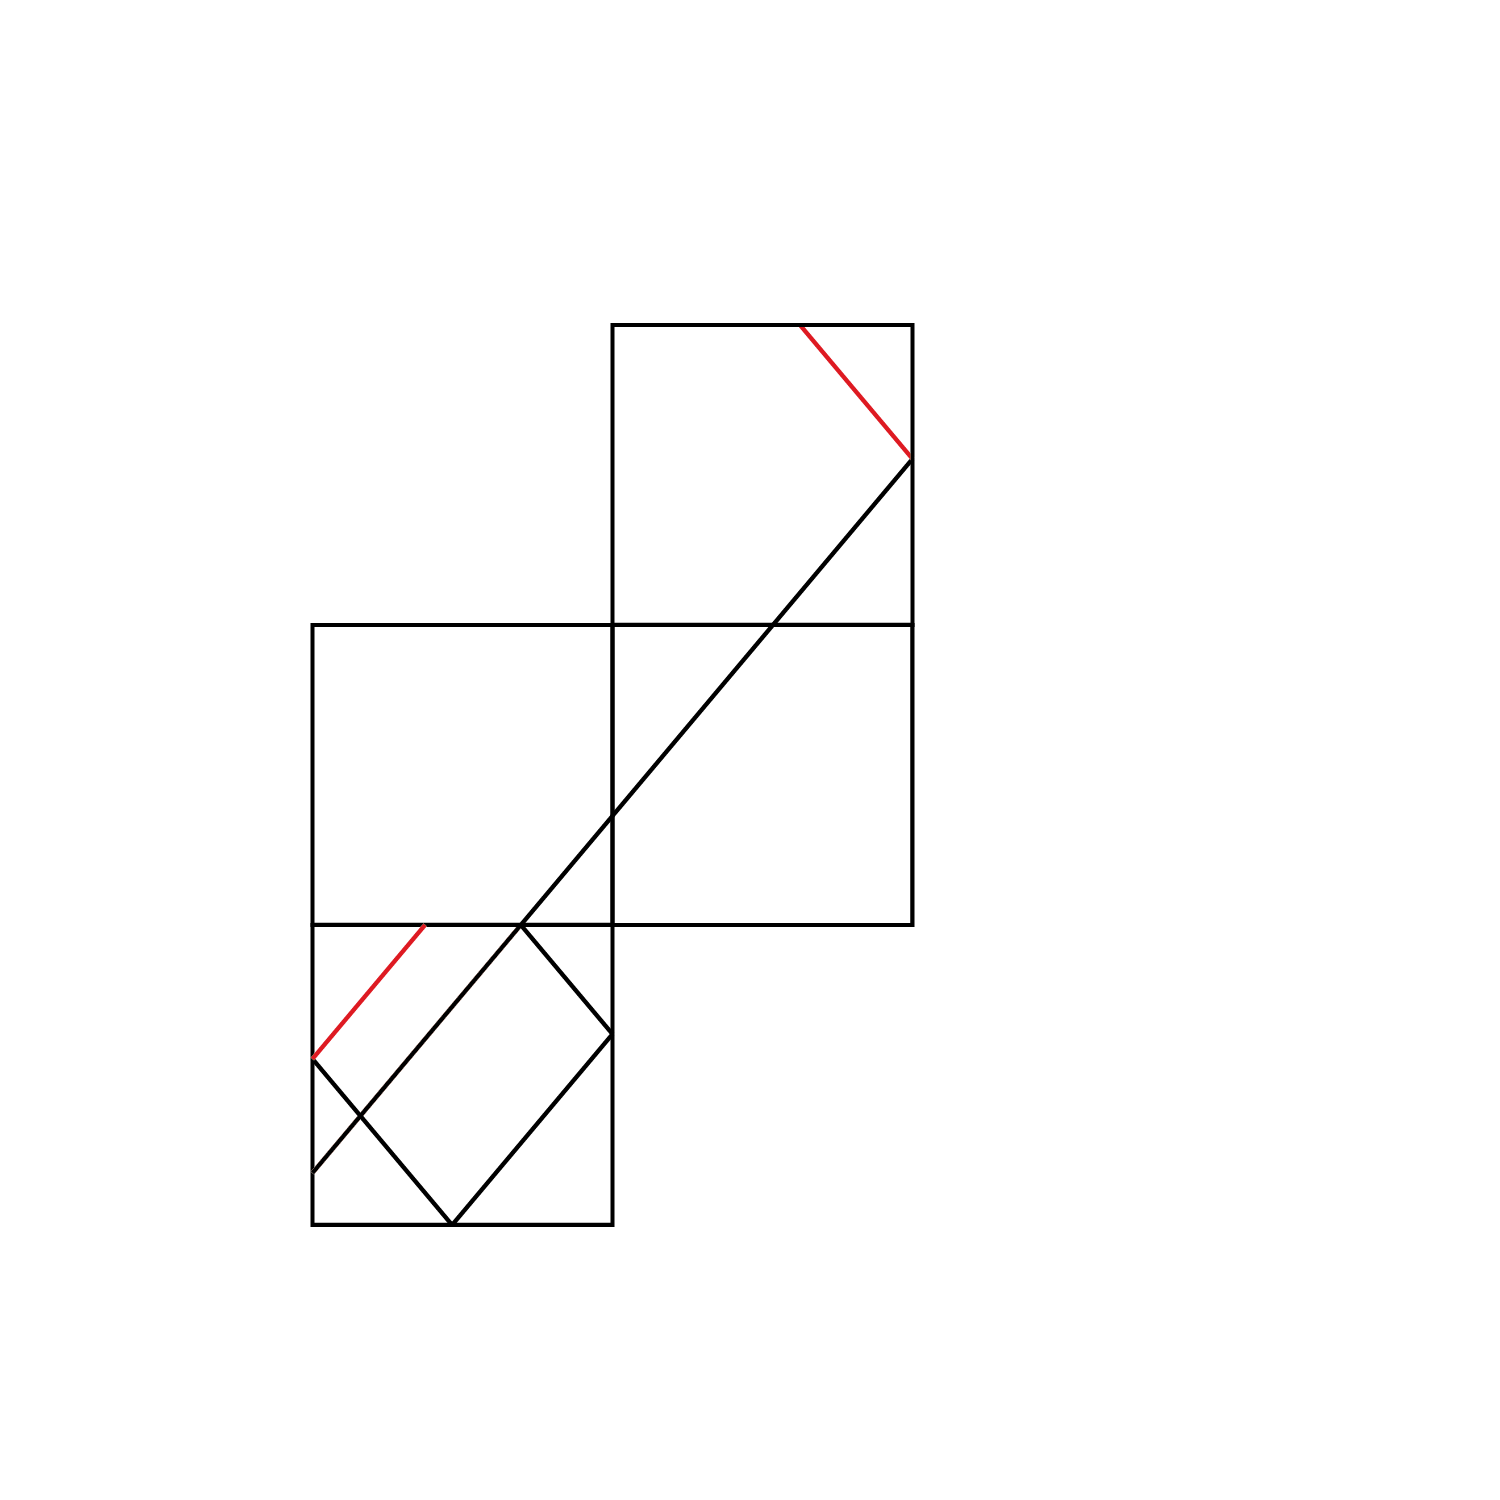
\includegraphics[width=3in]{tiling_(8)-01.png}
  \end{figure}
}
\frame{
  \frametitle{Tiling Tables}
  \begin{figure}
    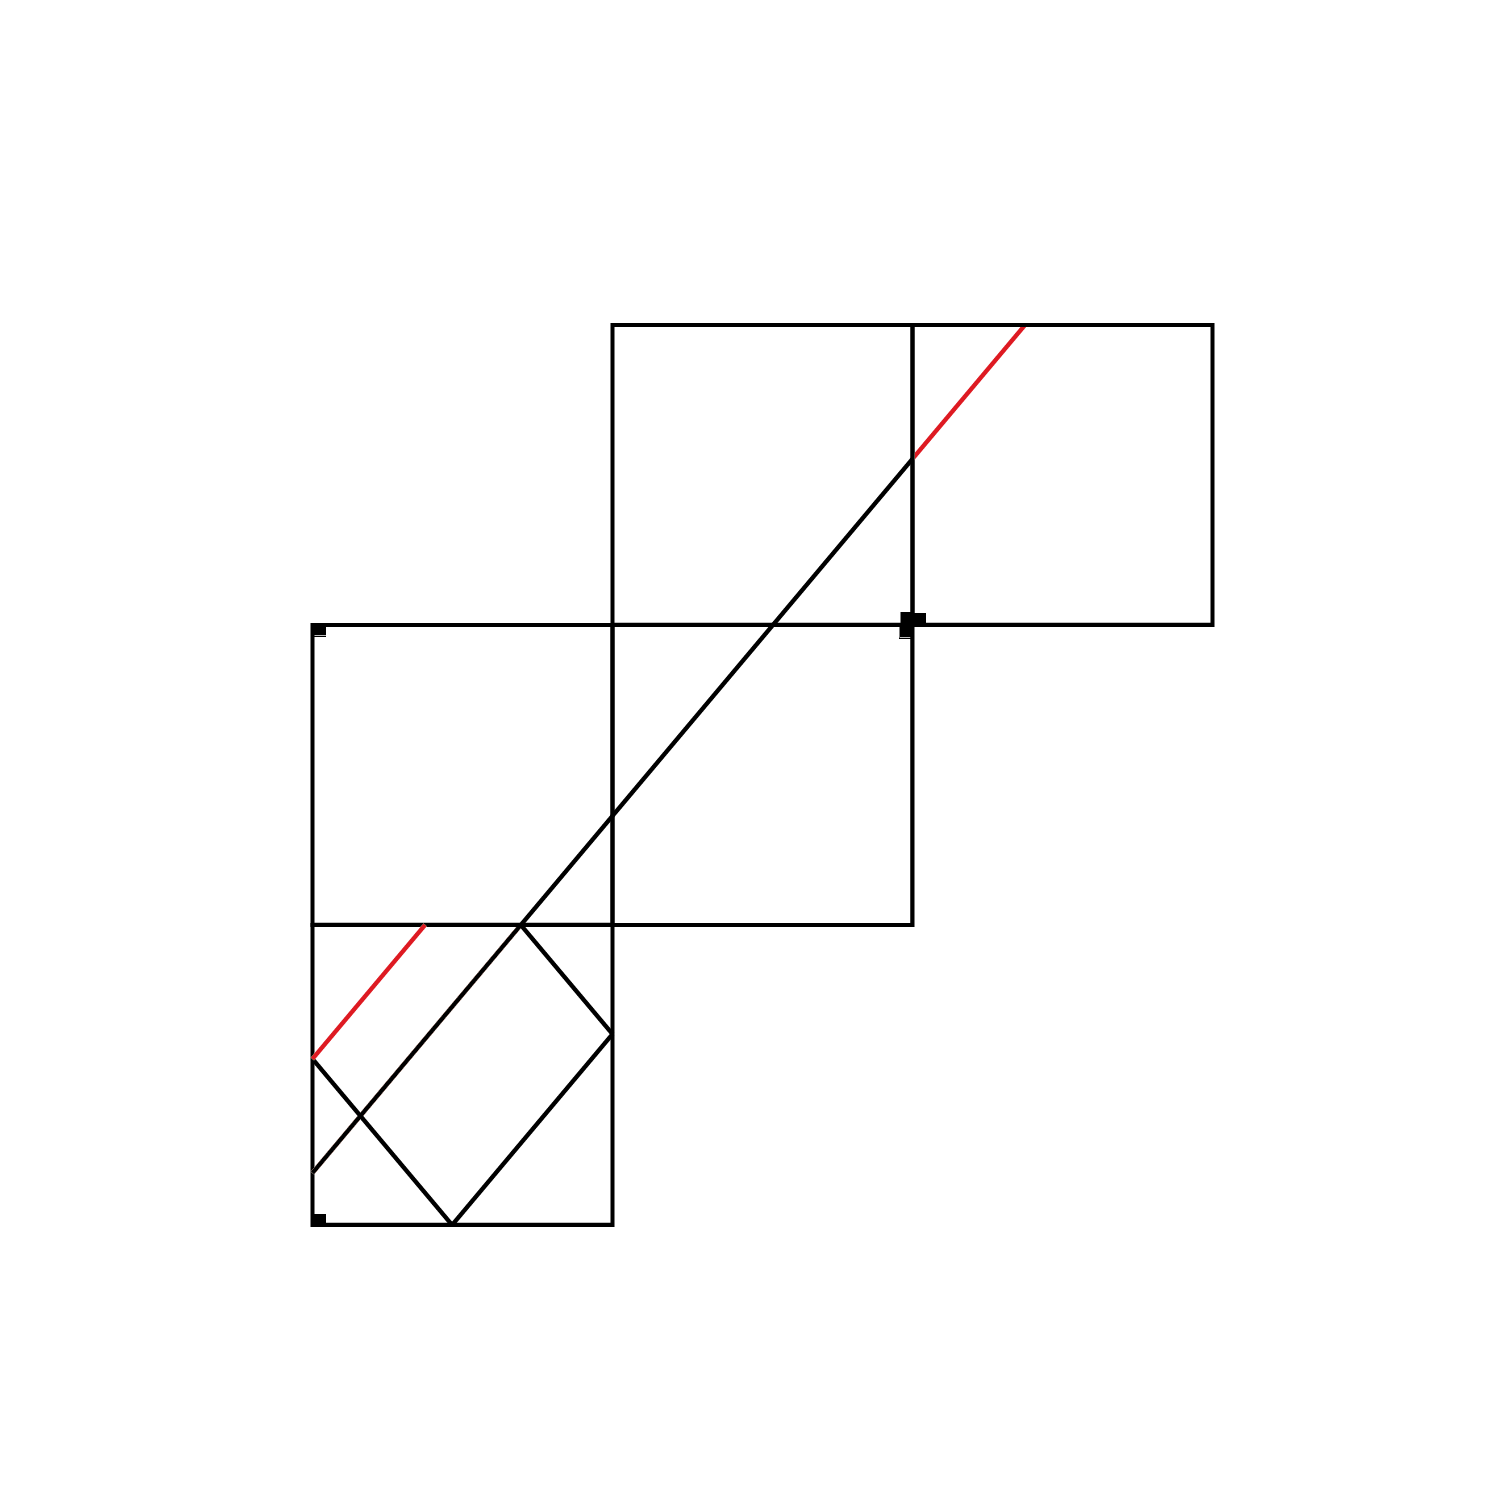
\includegraphics[width=3in]{tiling_(9)-01.png}
  \end{figure}
}
\frame{
  \frametitle{Tiling Tables}
  \begin{figure}
    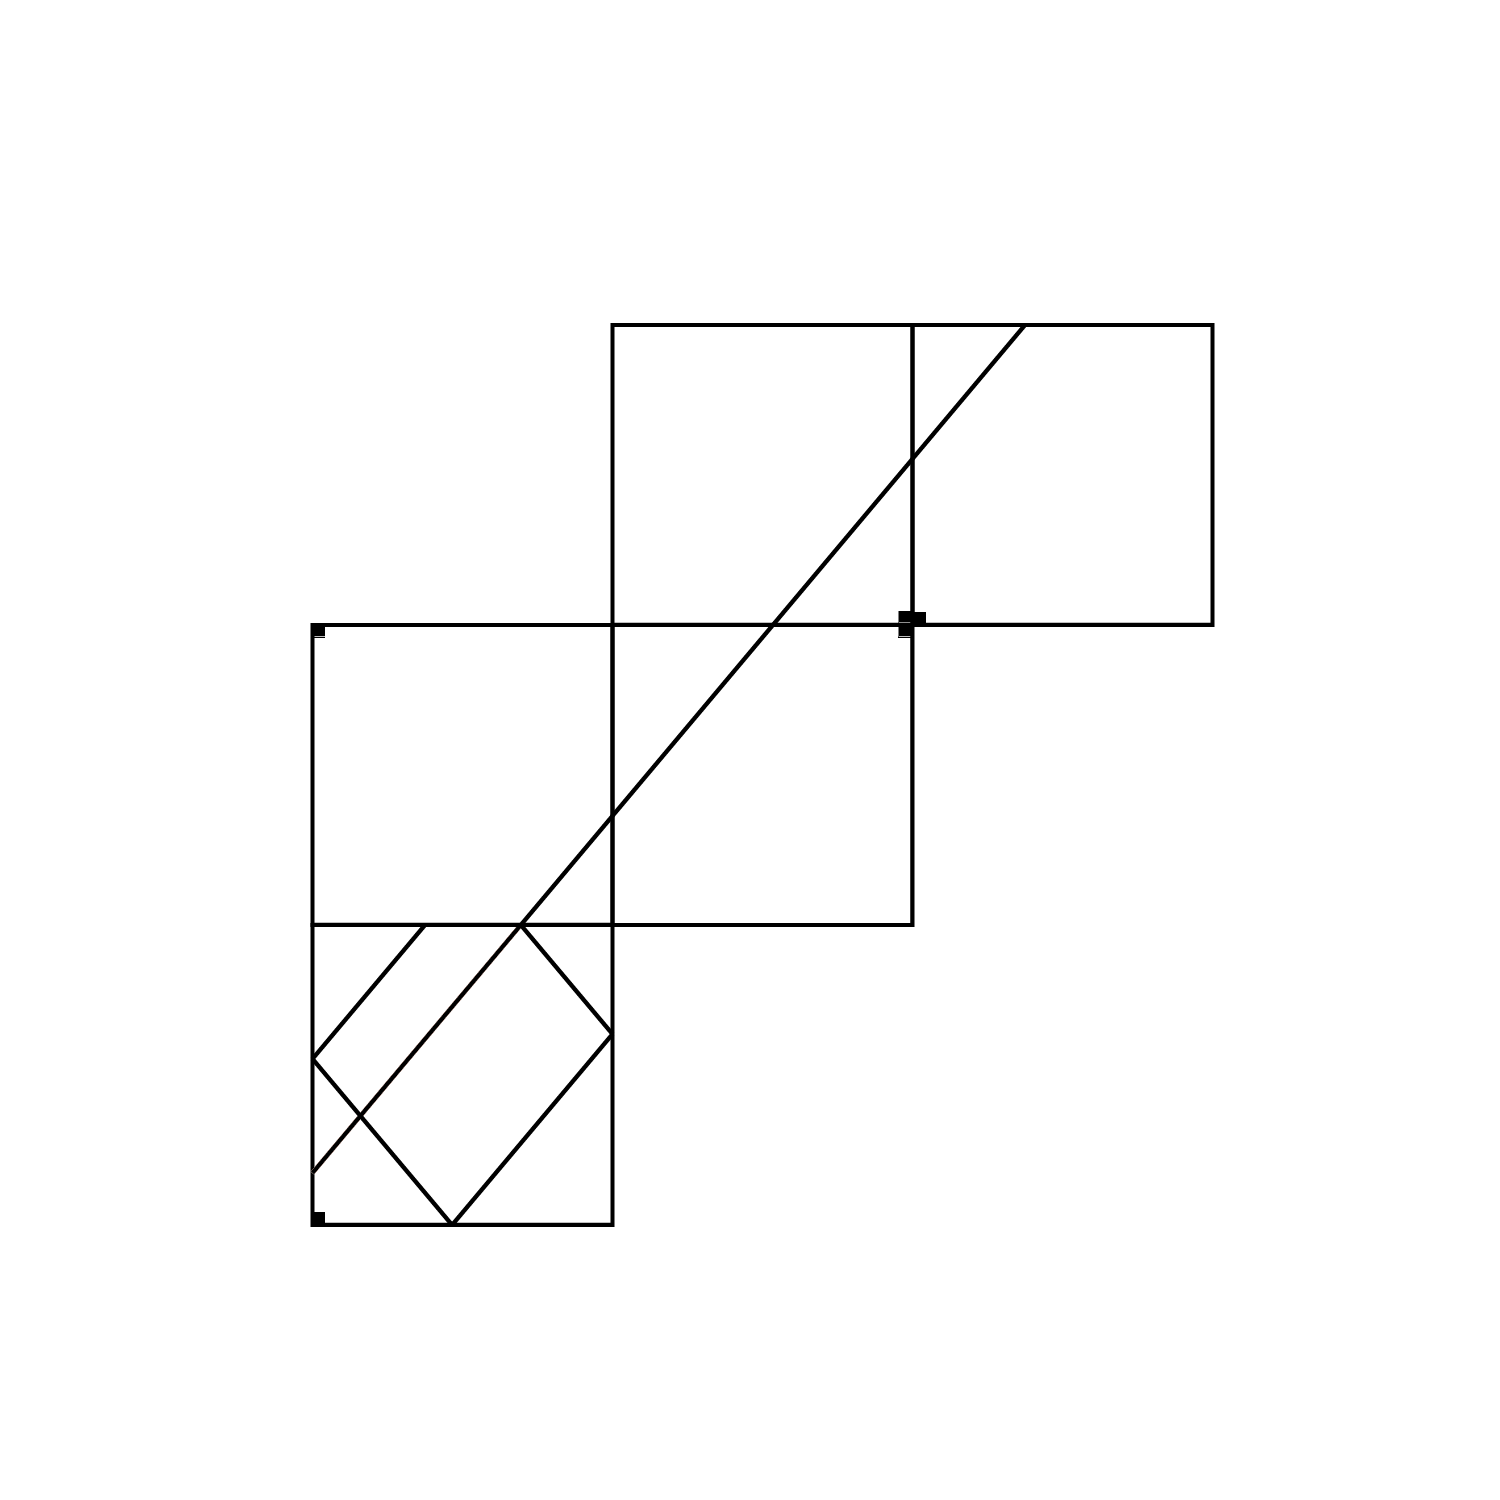
\includegraphics[width=3in]{tiling_(10)-01.png}
  \end{figure}
}
